%===============================================================================
\chapter{Identifica��o de sistemas}
\label{chapter:system_identification}
%===============================================================================

Neste capitulo ser� abordado uma breve introdu��o e apresenta��o sobre identifica��o de sistemas
lineares. Inicialmente ser� apresentado uma introdu��o com alguns dos principais fatos que motivam
a utiliza��o de identifica��o de sistemas (Se��o \ref{sec:sys_ident_objective}).

Em seguida ser� apresentado algumas das principais caracteristicas e o que comp�em a identifica��o de 
sistemas. Ser� descrito as principais caracteristicas e atribui��es do conjunto de dados 
utilizado para a identifica��o (se��o \ref{sec:sys_ident_data_acquisition}) e algumas das caracteristicas e 
utiliza��es do projeto de experimento (\ref{sec:si_project_experiments}).

Na se��o \ref{sec:sys_ident_modelling_choosing} ser� apresentado de forma sucinta algumas classes
mais comumente utlizadas para a modelagem de sistemas lineares. Em seguida ser� apresentado algumas
caracteristicas pertinentes a idenfica��o de sistemas com rela��o a propriedades das estimativas obtidas 
(\ref{sec:sys_ident_parameters_estimation}).

Ao fim ser� apresentado uma breve conclus�o sobre o que foi apresentado neste cap�tulo.

%===============================================================================
% Chapters
%===============================================================================
%===============================================================================
\section{Objetivo}
\label{sec:sys_ident_objective}
%===============================================================================

Identifica��o de sistemas possui uma vasta aplicabilidade em in�meros ramos do conhecimento,
n�o � escopo deste trabalho enumerar todas as possibilidades de utiliza��o desta ferramenta, nem t�o pouco 
esmiu�ar sua teoria. Ser� aqui abordado as principais caracter�sticas e princ�pios que comp�em a teoria de 
identifica��o de sistemas lineares.

O principal objetivo da identifica��o de um sistema � encontrar um modelo matem�tico que melhor consiga
descrever o sistema real sob observa��o, nas caracter�sticas desejadas escolhidas.

Pode-se considerar $y(t)$ como a sa�da do modelo matem�tico quando submetido a uma entrada $u(t)$ e
$\hat{y}(t)$ a sa�da real do sistema quando excitado pelo sinal de entrada $u(t)$. Os sinais $u(t)$
e $\hat{y}(t)$ s�o medidos pelo usu�rio.

Considerando o erro entre o sinal real $\hat{y}(t)$  e o sinal do modelo matem�tico $y(t)$ como:

\begin{equation}
\varepsilon (t)=y(t)-\hat{y}(t)
\nonumber
\end{equation}

A regress�o linear � o tipo mais simples de modelo param�trico. A estrutura do modelo
pode ser descrita como abaixo. \cite{system_identification}

\begin{equation}
y(t)=\varphi ^T(t)\theta
\label{eq:si_obj_single_var}
\end{equation}

Onde $y(t)$ � chamada de {\it{vari�vel regredida}} e � medida do processo.
$\varphi (t)$ � comumente chamado de {\it{vari�vel de regress�o}} e $\theta$ � o vetor de
par�metros.

Assim, o erro pode ser reescrito como:

\begin{equation}
\varepsilon (t)=y(t)-\varphi ^T(t)\theta
\nonumber
\end{equation} 

O objetivo da identifica��o de sistema, pode ser ent�o expresso como a escolha de um vetor $\hat{\theta}$ que
minimize a fun��o custo:

\begin{equation}
V(\theta)=\frac{1}{2}\sum_{t=1}^{N}\varepsilon ^2(t)=\frac{1}{2}\varepsilon^T\varepsilon=\frac{1}{2}\left \| \varepsilon \right \|
\label{eq:si_obj_etim_lsm_v}
\end{equation}

%===============================================================================
\subsection{Identificabilidade de sistemas}
\label{sec:si_par_estim_sys_ident}
%===============================================================================

A identificabilidade de um sistema pode ser definido pelo teorema (\ref{theorem:identificability}).

\begin{theorem} 
\cite{ljung}

Considerando a estrutura de modelo $\mathcal{M}$ correspondente a: 
\begin{equation}
A(q)y(t)=\frac{B(q)}{F(q)}u(t)+\frac{C(q)}{D(q)}e(t)
\label{eq:si_par_estim_sys_theorem}
\end{equation}

e com $\theta$ como em \eqref{eq:si_estim_predict_theta} sendo o coeficiente dos polin�mios envolvidos.
Os graus dos polin�mios s�o $n_a$, $n_b$ e assim por diante. A estrutura deste modelo 
� globalmente identific�vel se, e somente se, todos os itens de (i) at� (vi) forem verdadeiros.

\begin{enumerate}[(i)]
\item N�o existe fator comum para todos os $z^{na}A^*(z), z^{nb}B^*(z), and, \; z^{nc}C^*(z)$.
\item N�o existe fator comum para $z^{nb}B^*(z), and, \; z^{nf}F^*(z)$.
\item N�o existe fator comum para $z^{nc}C^*(z), and, \; z^{nd}D^*(z)$.
\item Se $n_a \geq 1$ ent�o n�o pode existir fator comum entre $z^{nf}F^*(z), and, \; z^{nd}D^*(z)$.
\item Se $n_d \geq 1$ ent�o n�o pode existir fator comum entre $z^{na}A^*(z), and, \; z^{nb}B^*(z)$.
\item Se $n_f \geq 1$ ent�o n�o pode existir fator comum entre $z^{na}A^*(z), and, \; z^{nc}C^*(z)$.
\end{enumerate}

Os polin�mios com $*$ correspondem a $\theta^*$
\label{theorem:identificability}
\end{theorem}

Note que as condi��es de (i) at� (vi) s�o satisfeitas para o caso comum de \eqref{eq:si_par_estim_sys_theorem}.
Observe tamb�m que nenhuma das condi��es pode ser violada por qualquer {\it{especial}} valor de $\theta^*$, posto na
hiper-superf�cie de $\Re ^d$. Isso nos leva ao seguinte corol�rio:

\begin{cor} 
A estrutura de modelo apresentada em \eqref{eq:si_par_estim_sys_theorem} � globalmente identific�vel.
\label{corollary:identificability}
\end{cor} 

A partir do Corol�rio (\ref{corollary:identificability}) temos que a identifica��o de sistemas
utilizando os modelos descritos pela Tabela \ref{table:si_modeling_models} s�o globalmente identific�veis
se tivermos os dados de entrada suficientemente informativos.


%===============================================================================
\section{Conjunto de dados coletados}
\label{sec:sys_ident_data_acquisition}
%===============================================================================

Identifica��o de sistemas � baseada no conjunto de dados coletados do sistema
observado. Estes dados podem ser obtidos em regime normal de opera��o ou sob
condi��es pr� determinadas, onde � poss�vel escolher previamente o sinal de
entrada que ser� aplicado sobre o sistema. Isso � feito para que os dados
coletados sejam o mais informativos poss�veis. \cite{ljung} Maiores detalhes
sobre escolha de sinais para alimenta��o ser�o abordados no capitulo sobre 
projeto de experimentos (se��o (\ref{sec:si_project_experiments})).

Um conjunto de dados obtidos tanto por malha aberta quanto por malha fechada
pode ser descrito como em \eqref{eq:si_data_acq}. 

\begin{equation}
z^N=\left \{  u(1), y(1), ... ,u(N), y(N) \right \}
\label{eq:si_data_acq}
\end{equation}

%===============================================================================
\subsection{Persist�ncia de Excita��o}
\label{sec:si_data_persistently_excitation}
% most part of it came from ljung pg 412
%===============================================================================

Um sinal persistentemente excitante com rela��o ao modelo $\mathcal{M}^*$ significa que 
os dados coletados permitem a discrimina��o entre dois modelos diferentes dentro do modelo
$\mathcal{M}^*$.

Um sinal quasi-estacion�rio $\left \{ u(t) \right \}$, com espectro $\Phi _u(\omega)$ � dito
{\it{persistentemente excitante de ordem n}} se, para todos os filtros de forma:

\begin{equation}
M_n(q)=m_1q^{-1}+...+m_nq^{-n}
\label{eq:si_data_persistence}
\end{equation}

a rela��o

\begin{equation}
\left | M_n(e^{i\omega}) \right |^2 \Phi_u(\omega)\equiv 0, \;\; \text{implica que}\; M_n(e^{i\omega}) \equiv 0
\label{eq:si_data_persistence_2}
\end{equation}

Outra caracteriza��o pode ser dada em termos da fun��o de covari�ncia $R_u(\tau)$= $u(t)$ � um
sinal quasi-estacion�rio, e $\bar{R}_n$ uma matriz $n\times n$ definida como:

\begin{equation}
\bar{R}_n=\begin{bmatrix}
R_u(0) & R_u(1) & ... & R_u(n-1)\\ 
R_u(1) & R_u(2) & ... & R_u(n-2)\\ 
\vdots & \vdots & \vdots & \vdots \\ 
R_u(n-1) & R_u(n-2) & ... & R_u(0)
\end{bmatrix}
\label{eq:si_data_persistently_rn}
\end{equation}

Ent�o $u(t)$ � persistentemente excitante de ordem $n$ se e somente se, $\bar{R}_n$ for n�o singular.
\cite{ljung}

A partir da equa��o \eqref{eq:si_data_persistence_2} pode-se extrair interpreta��es mais explicitas.
Uma delas � que a fun��o $M_n(z)M_n(z^{-1})$ pode ter no m�ximo $n-1$ polos diferentes dentro do circulo 
unit�rio (desde que um zero esteja sempre na origem) levando a simetria em conta. Por isso $u(t)$ �
persistentemente excitante de ordem $n$, se o espectro do sinal de entrada, $\Phi _u(\omega)$, for
diferente de de zero em pelo menos $n$ pontos no intervalo $-\pi< \omega \le \pi$. \cite{ljung}

Considere o somat�rio de senoides em \eqref{eq:si_data_persistently_sum_cos}, cada senoide possui duas
linhas espectrais em $\pm \omega_k$. Este sinal � ent�o persistentemente excitante de ordem $2n$.

\begin{equation}
u(t)=\sum_{k=1}^{n}\mu_k \cos (\omega_kt), \;\; \omega_k \neq \omega_j, \;\; \omega_k \neq 0, \; \omega_k \neq \pi
\label{eq:si_data_persistently_sum_cos}
\end{equation}

%===============================================================================
\subsection{Experimentos Informativos}
% most part of it came from ljung pg 414
%===============================================================================

Na Se��o \ref{sec:si_data_persistently_excitation} foi visto que � f�cil caracterizar
sinais que s�o suficientemente informativos.Considere um conjunto $\mathcal{M}^*$ de um modelo
SISO descrito por (\ref{eq:si_data_model_def}) tendo a fun��o de transfer�ncia $G(q,\theta)$ a
fun��o racional descrita em (\ref{eq:si_data_g_rational}).

\begin{equation}
\mathcal{M}^*=\left \{ G(q,\theta), H(q,\theta)|\theta \in D_{\mathcal{M}} \right \}
\label{eq:si_data_model_def}
\end{equation}

\begin{equation}
G(q,\theta)=\frac{B(q,\theta)}{F(q,\theta)}=\frac{q^{n_k}(b_1+b_2q^{-1}+...+b_{nb}q^{-nb+1})}{1+f_1q^{-1}+...+f_{nf}q^{-nf}}
\label{eq:si_data_g_rational}
\end{equation}

Ent�o um experimento em malha aberta com uma entrada que � persistentemente excitante de ordem $nb +nf$ �
suficientemente informativo com rela��o a $\mathcal{M}^*$.

Um experimento em malha aberta � informativo se a sua entrada for persistentemente excitante.
Observa-se que � necess�rio que a ordem de excita��o seja igual ao n�mero de par�metros a
serem estimados. \cite{ljung}



\section{Modelagem de Sistemas}
\label{sec:sys_ident_modeling}
%===============================================================================

Sistemas existem em toda nossa volta, podem ser simples, complexos, podemos percebe-los como um sistema
ou podemos nem perceber que estamos interagindo com um. Ao dirigir um carro por exemplo, constru�mos um
modelo mental para o sistema que � o carro e por meio das percep��es que temos agimos sobre o sistema
a fim de controla-lo da forma como desejamos.

Modelos s�o formas ou representa��es de como vemos e entendemos os sistemas. Para um mesmo sistema podemos ter
diversos modelos. No caso de dirigir um carro, por exemplo, estamos mais acostumados a dirigir um carro em 
especifico. Ao trocar de carro, passamos a ter a percep��o de que alguma coisa n�o esta funcionando corretamente, 
a resposta da acelera��o, embreagem � diferente. Desta forma o modelo mental que temos para o nosso carro n�o 
� 100 \% compat�vel com o novo carro, devemos ent�o adequar nosso modelo mentar � resposta do novo carro aos
nossos comandos.

Modelos, portanto, s�o fundamentais para o conhecimento, para a an�lise, para o controle de sistemas. \cite{aguirre}.
A modelagem do processo de dirigir � um modelo mental, existem outros tipos de modelos para sistemas que s�o
mais consistentes e podem ser difundidos e compartilhados entre as pessoas sem haver a necessidade de entender 
o que a pessoa formulou mentalmente para o sistema. Modelos que possam se relacionar de forma matem�tica s�o
de grande apelo, e assim como os modelos mentais, modelos matem�ticos tamb�m s�o formados por por observa��o
e dados coletados que descrevem o funcionamento do sistema.

Existem dois principais ramos para modelagem de sistemas, um deles parte-se do conhecimento intr�nseco do mesmo
para obter-se o modelo, enquanto que o outro n�o possui este pr�-requisito, focando-se em t�cnicas que tornem o
processo de modelagem o mais independente poss�vel da necessidade de se conhecer o sistema, antes de modela-lo. 
Estes dois processos s�o conhecidos como {\it{Modelagem caixa branca}} e {\it{Modelagem caixa preta}} respectivamente.

No caso de modelagem caixa branca, faz-se necess�rio conhecer a fundo o sistema modelado. Al�m de estar bem 
familiarizado cm o sistema � necess�rio conhecer as rela��es matem�ticas que descrevem os fen�menos envolvidos.
Modelagem caixa branca tamb�m � conhecida como {\it{Modelagem pela F�sica}}, {\it{Natureza do processo}} ou 
{\it{conceitual}}. Para uma modelagem caixa branca normalmente gasta-se um elevado tempo para que todos os 
fen�menos envolvidos sejam conhecidos e caracterizado, devido a isso nem sempre � vi�vel seguir este procedimento.
\cite{aguirre}.

Identifica��o de sistemas � uma �rea do conhecimento que estuda t�cnicas alternativas para modelagem matem�tica.
Uma das caracter�sticas destas t�cnicas � que pouco ou nenhum conhecimento pr�vio do sistema � necess�rio. Este tipo 
de t�cnica � tamb�m conhecido como {\it{Modelagem (ou identifica��o) caixa preta}} ou {\it{modelagem emp�rica}}.

Algo importante a se destacar antes do processo de modelagem do sistema � a escolha do que deseja-se modelar deste
sistema. Uma modelagem completa de todas as caracter�sticas � muitas vezes invi�vel e na maioria dos sistemas reais, 
desnecess�rio. Usualmente, temos a necessidade de interagir, seja controlando ou observando, um conjunto restrito 
de informa��es do sistema. No exemplo de dirigir, n�o necessidade de que seja modelado a transfer�ncia de calor do 
motor, este tipo de informa��o n�o ajudaria no processo de dirigir o carro, podendo ser desconsiderado da modelagem.


\subsection{Considera��es em modelagem}
\label{sec:sys_ident_basic_definitions}
%===============================================================================

Geralmente, na modelagem de sistemas, fazem-se algumas considera��es sobre o sistema:

{\it{Linearidade}}. Uma considera��o frequentemente feita � a de se supor que o sistema sendo modelado se comporta 
de forma aproximadamente linear. Tal suposi��o � normalmente verificada observando-se o comportamento em uma faixa
relativamente estreita de opera��es. \cite{aguirre}

Formalmente diz-se que um sistema � linear se ele obedece o {\it{principio da superposi��o}} [todo:achar a bibliografia disso].
A considera��o da linearidade normalmente simplifica bastante p modelo a ser constru�do. Entretanto, h� situa��es em que 
esta considera��o n�o � adequada, como por exemplo, para sistemas como din�mica fortemente bilinear (que n�o podem ser descritos
adequadamente por um �nico modelo linear, independentemente de qu�o estreita seja a faixa de opera��o considerada). E tamb�m
no caso onde se deseja estudar caracter�sticas din�micas n�o-lineares do sistema, tais como oscila��es e bifurca��es.
\cite{aguirre}

{\it{Invari�ncia no tempo}}. A considera��o de invari�ncia temporal implica que o comportamento do sistema sendo modelado n�o 
varia com o tempo. Isso n�o significa que as vari�veis do sistema tenham valores constantes. Pelo contrario, normalmente os
valores das vari�veis que caracterizam um sistema flutuam com o tempo, sendo que tal evolu��o temporal � determinada por uma 
lei. Normalmente refere-se a esta lei como a din�mica do sistema. Portanto, ser invariante no tempo n�o quer dizer que o sistema
esta est�tico, mas certamente implica que a din�mica que esta regulando a evolu��o temporal e a mesma. 

Formalmente diz-se que um sistema � invariante se um deslocamento no tempo na entrada causa um deslocamento no tempo na sa�da.

\subsection{Forma geral de familias de modelos}
\label{sec:si_modeling_family_models}
%===============================================================================

Como j� foi dito, o modelo de um sistema � a descri��o de algumas propriedades deste. Nesta se��o ser� 
apresentado modelos de sistemas invariantes no tempo.

Um modelo linear pode ser representado como em (\ref{eq:si_modeling_lti}).

\begin{equation}
y(t)=G(q)u(t)+H(q)e(t)
\label{eq:si_modeling_lti}
\end{equation}

com:

\begin{equation}
G(q)=\sum_{k=1}^{\infty}g(k)q^{-k}\\
\\
H(q)=1+\sum_{k=1}^{\infty}h(k)q^{-k}
\label{eq:si_modeling_lti_det}
\end{equation}

Uma forma bem direta para a identifica��o de sistemas � tornar as fun��es $G(q)$ e $H(q)$ de (\ref{eq:si_modeling_lti_det})
como fun��es racionais e que os coeficientes do denominador e numerador destes polinimios sejam os objetivos do processo
de identifica��o.

%===============================================================================
\section{Estimativa de par�metros}
\label{sec:sys_ident_parameters_estimation}
%===============================================================================

A estimativa dos par�metros dos modelos dependem de v�rios fatores, at� agora foi apresentado
a import�ncia dos dados coletados (Se��o (\ref{sec:sys_ident_data_acquisition})) e da 
escolha do modelo (Se��o (\ref{sec:sys_ident_modelling_choosing})). Nesta se��o ser�o 
apresentados algumas formas para a estimativa dos par�metros, bem como algumas de suas
caracter�sticas probabil�sticas. 

A identifica��o � baseada em um conjunto de dados coletados do sistema, um modelo para caracteriza-lo.
Um preditor � uma equa��o que tenta prever o pr�ximo valor do sistema baseado nos dados passados deste.
Com o preditor atinge-se um conjunto de dados que deve ser muito pr�ximo aos dados verdadeiros
coletados do sistema. Escolhe-se ent�o um m�todo para minimiza��o do erro existente entre
os dados coletados e os dados calculados pelo preditor.

Por fim ser� apresentado algumas das caracter�sticas para a estima��o quando alguns 
requisitos para a identifica��o n�o n�o atingidos, como por exemplo quando o modelo
escolhido n�o consegue representar o sistema, ou quando o dados de entrada n�o s�o 
suficientemente informativos. Nestas situa��es teremos erros na estimativa dos par�metros.
Erros diferentes que ser�o abordados na se��o (\ref{sec:si_par_estim_uncertanties}).


%===============================================================================
\subsection{Preditores}
\label{sec:si_par_estim_preditors}
% ljung pg 68
%===============================================================================

Preditores s�o equa��es que tentam prever qual ser� o pr�ximo valor de sa�da do sistema
baseado no modelo deste e nos valores de dados coletados at� aquele momento.
Considere o sistema apresentado em (\ref{eq:si_modeling_lti}). Assume-se que os
sinais $y(p)$ e $u(p)$ s�o conhecidos para $p \le t-1$. A partir de (\ref{eq:si_par_estim_vs})
tem-se que at� $\upsilon (p)$ � definido. O objetivo ent�o � prever $y(t)$ como
em (\ref{eq:si_par_estim_yt}).

\begin{equation}
\upsilon (p)=y(p) -G(q)u(p)
\label{eq:si_par_estim_vs}
\end{equation}

\begin{equation}
y(t)=G(q)u(t)+\upsilon (t)
\label{eq:si_par_estim_yt}
\end{equation}

Fazendo-se as substitui��es necess�rias chega-se ao estimador (\ref{eq:si_par_estim_predictor})
onde enfatiza-se a depend�ncia com o par�metro $\theta$ \cite{ljung}. Este preditor tamb�m
� conhecido como preditor �timo, sendo utilizado em diversos m�todos de identifica��o de
sistemas.

\begin{equation}
\hat{y}(t|\theta)=H^{-1}(q,\theta)G(q,\theta)u(t)+\left [ 1- H^{-1}(q,\theta)\right ]y(t)
\label{eq:si_par_estim_predictor}
\end{equation}

O erro de predi��o � a diferen�a entre os valores atingido pelo preditor e os valores 
reais coletados do sistema como apresentado em \eqref{eq:si_par_estim_err_predic}.
Este erro � amplamente utilizado para determinar a qualidade da estimativa que se 
encontra. Como ser� visto a seguir.

\begin{equation}
\varepsilon (t| \theta)=y(t)-\hat{y}(t|\theta)
\label{eq:si_par_estim_err_predic}
\end{equation}

Onde $y(t)$ s�o os dados coletados do sistema e $\hat{y}(t|\theta)$ os dados provenientes da 
estimativa. A equa��o do erro (\eqref{eq:si_par_estim_err_predic} pode ser reescrita como:

\begin{equation}
\varepsilon (t,\theta)=\frac{D(q)}{C(q)}\left [ A(q)y(t) - \frac{B(q)}{F(q)}u(t)\right ]
\nonumber
\end{equation}

Definimos ent�o duas vari�veis auxiliares \eqref{eq:si_estim_predict_w} e \eqref{eq:si_estim_predict_v}

\begin{equation}
w(t,\theta)=\frac{B(q)}{F(q)}u(t)
\label{eq:si_estim_predict_w}
\end{equation}

\begin{equation}
\upsilon (t,\theta)=A(q)y(t)-w(t,\theta)
\label{eq:si_estim_predict_v}
\end{equation}

Ent�o:

\begin{equation}
\varepsilon (t,\theta)=y(t)-\hat{y}(t|\theta)=\frac{D(q)}{C(q)}\upsilon (t,\theta)
\nonumber
\end{equation}

Desta forma introduz-se o vetor de estados \eqref{eq:si_estim_predic_state}.\cite{ljung}

\begin{equation}
\begin{matrix}
\varphi (t,\theta)= & [ -y(t-1), ... , -y(t-n_a), u(t-1), ..., u(t-n_b),\\ 
 & -w(t-1, \theta),..., -w(t-n_f, \theta), \varepsilon (t-1, \theta), ...,\varepsilon (t-n_c, \theta),\\ 
 & \upsilon (t-1, \theta), ...,\upsilon (t-n_d, \theta) ]^T
\end{matrix}
\label{eq:si_estim_predic_state}
\end{equation}

E o vetor de par�metros \eqref{eq:si_estim_predict_theta}:

\begin{equation}
\theta = \left [ a_1 \; ... \; a_{na} \; b_1 \; ... \; b_{nb} \; f_1 \; ... \; f_{nf} \; c_1 \; ... \; c_{nc} \; d_1 \; ... \; d_{nd}\right ]^T
\label{eq:si_estim_predict_theta}
\end{equation}

Chega-se ent�o a seguinte equa��o para o erro de predi��o:

\begin{equation}
\varepsilon (t,\theta)=y(t)-\theta^T\varphi (t,\theta)
\label{eq:si_estim_predict_erro}
\end{equation}

Onde:

\begin{equation}
\hat{y}(t| \theta)=\theta^T\varphi (t,\theta)=\varphi ^T(t,\theta)\theta
\nonumber
\end{equation}

%===============================================================================
\subsection{M�todo dos m�nimos quadrados}
\label{sec:si_par_estim_lsm}
%===============================================================================

Existem diversos m�todos para a estimativa de par�metros. O mais conhecido, remete
ao ano de 1809 utilizado por Gauss para determina��o da orbita dos planetas. 
\cite{system_identification}. M�todo este chamado de M�todo dos m�nimos quadrados (MMQ).

A regress�o linear � o tipo mais simples de modelo param�trico. A estrutura do modelo
pode ser descrita como em (\ref{eq:si_lsm_single_var}).

\begin{equation}
y(t)=\varphi ^T(t)\theta
\label{eq:si_lsm_single_var}
\end{equation}

Onde $y(t)$ � chamada de {\it{vari�vel regredida}} e � medida do processo.
$\varphi (t)$ � comumente chamado de {\it{vari�vel de regress�o}} e $\theta$ � o vetor de
par�metros.

O modelo apresentado em (\ref{eq:si_lsm_single_var}) � facilmente estendido para o modelo
multivari�veis (\ref{eq:si_lsm_multi_var}).

\begin{equation}
y(t)=\Phi ^T(t)\theta
\label{eq:si_lsm_multi_var}
\end{equation}

Onde $y(t)$ � um vetor de $p$ posi��es, $\Phi(t)$ uma matriz $n \times p$ e $\theta$ � um 
vetor de $N$ posi��es.

A ideia do m�todo � encontrar uma estimativa $\hat{\theta}$ dos par�metros de $\theta$ a partir de medidas
de $y(1),\varphi(1),\cdots,y(N),\varphi(N)$. 

A partir de (\ref{eq:si_par_estim_err_predic}) e (\ref{eq:si_lsm_single_var}) temos 

\begin{equation}
\varepsilon (t)=y(t)-\varphi ^T(t)\theta
\nonumber
\end{equation}

A {\it{estimativa dos m�nimos quadrados}} de $\theta$ � definido como o vetor $\hat{\theta}$ 
que minimiza a fun��o custo (\ref{eq:si_par_etim_lsm_v}). Este � o crit�rio de minimiza��o do 
erro de predi��o para o m�todo dos m�nimos quadrados.

\begin{equation}
V(\theta)=\frac{1}{2}\sum_{t=1}^{N}\varepsilon ^2(t)=\frac{1}{2}\varepsilon^T\varepsilon=\frac{1}{2}\left \| \varepsilon \right \|
\label{eq:si_par_etim_lsm_v}
\end{equation}

O valor de $\hat{\theta}$ que minimiza (\ref{eq:si_lsm_single_var}) � dado por:

\begin{equation}
\hat{\theta}=(\varphi ^T \varphi )^{-1}\varphi  ^T y
\label{eq:si_par_etim_lsm_theta}
\end{equation}

O m�nimo da fun��o custo fica como em:

\begin{equation}
\underset{\theta}{min}\;V(\theta)=V(\hat{\theta})=\frac{1}{2}\left [ y^Ty-y^T\varphi (\varphi ^T \varphi )^{-1}\varphi ^T y \right ]
\end{equation}

%===============================================================================
\subsection{M�todo das vari�veis instrumentais}
\label{sec:si_par_estim_iv}
%===============================================================================
% bibliografia principal: aguirre e ljung

O m�todo dos m�nimos quadrados apresentados na se��o (\ref{sec:si_par_estim_lsm}) �
simples de ser aplicado, mas tem o inconveniente de que para que n�o existam erros de 
polariza��o na estimativa, a vari�vel de regress�o $\phi(t)$ n�o pode estar
correlacionada com o dist�rbio estoc�stico $\nu(t)$. Assume-se que o sistema real � dado
por:

\begin{equation}
y(t)=\varphi^T(t)\theta_0+\nu(t)
\label{eq:si_par_etim_iv_true_sys}
\end{equation}

No m�todo dos m�nimos quadrados $\varphi(t)$ depende da sa�da e implicitamente dos valores passados
de $\nu(t)$, desta forma \eqref{eq:si_par_etim_iv_estim} seria bem restritivo, mas de fato o que
pode ser demonstrado � que \eqref{eq:si_par_etim_iv_estim} � satisfeito somente se $\nu(t)$
for ruido branco. Esta desvantagem do m�todo dos m�nimos quadrados pode ser visto como uma
vantagem para a introdu��o do m�todo de vari�veis instrumentais. \cite{system_identification}

\begin{equation}
E(\varphi(t) \; \nu(t)) = 0
\label{eq:si_par_etim_iv_estim}
\end{equation}

Assume-se que $Z(t)$ � uma matriz $n\times n$ que possuem sinais n�o correlacionados com o 
dist�rbio $\nu(t)$. O par�metro $\theta$ deve obedecer a restri��o da equa��o \eqref{eq:si_par_estim_iv_theta}:

\begin{equation}
\frac{1}{N}\sum_{t=1}^{N}Z(t)\varepsilon (t)=\frac{1}{N}\sum_{t=1}^{N}Z(t)\left [ y(t)-\varphi^T(t)\theta \right ]= 0
\label{eq:si_par_estim_iv_theta}
\end{equation}

Se a dimens�o da matriz $Z(t)$ for a mesma dimens�o de $\theta$ temos o estimados dos m�todo de 
vari�veis instrumentais \eqref{eq:si_par_estim_iv}:

\begin{equation}
\hat{\theta}=\left [ \sum_{t=1}^{N}Z(t)\varphi^T(t) \right ]^{-1}\left [  \sum_{t=1}^{N}Z(t)y(t) \right ]
\label{eq:si_par_estim_iv}
\end{equation}

Os elementos da matriz $Z(t)$ s�o normalmente chamados de instrumentos. O estimador das vari�veis instrumentais 
� uma generaliza��o do estimador dos m�nimos quadrados, quando $Z(t)=\varphi(t)$. \cite{system_identification}

O estimador de vari�veis instrumentais evita a polariza��o garantido  que o vetor de erro seja n�o correlacionado
com as vari�veis instrumentais. Esta condi��o e menos restritiva que a condi��o dos m�nimos quadrados para que
n�o haja erro de polariza��o \eqref{eq:si_par_etim_iv_estim}. O valor a ser pago por isso envolve: \cite{aguirre}

\begin{enumerate}[(I)]
\item Escolha das vari�veis instrumentais.
\item O estimador resultante � assintoticamente n�o polarizado, ao inv�s de ser apenas n�o polarizado.
\end{enumerate}

Ao escolher as vari�veis instrumentais � importante notar que a escolha n�o deve ser apenas para evitar 
a correla��o entre o vetor de erro e os instrumentos. A raz�o para isso � que as vari�veis instrumentais 
devem ser t�o correlacionadas quanto poss�vel com os regressores do modelo, caso contr�rio $Z(t)\varphi(t)^T$ 
seria pr�xima a singular e sua inversa muito mal condicionada. Portanto os instrumentos devem ser, idealmente, 
pouco correlacionados com o erro e muito correlacionados com os regressores do modelo. \cite{aguirre}


%===============================================================================
\subsection{Identificabilidade de sistemas}
\label{sec:si_par_estim_sys_ident}
%===============================================================================

A identificabilidade de um sistema pode ser definido pelo teorema (\ref{theorem:identificability}).

\begin{theorem} 
\cite{ljung}

Considerando a estrutura de modelo $\mathcal{M}$ correspondente a: 
\begin{equation}
A(q)y(t)=\frac{B(q)}{F(q)}u(t)+\frac{C(q)}{D(q)}e(t)
\label{eq:si_par_estim_sys_theorem}
\end{equation}

e com $\theta$ como em \eqref{eq:si_estim_predict_theta} sendo o coeficiente dos polin�mios envolvidos.
Os graus dos polin�mios s�o $n_a$, $n_b$ e assim por diante. A estrutura deste modelo 
� globalmente identific�vel se, e somente se, todos os itens de (i) at� (vi) forem verdadeiros.

\begin{enumerate}[(i)]
\item N�o existe fator comum para todos os $z^{na}A^*(z), z^{nb}B^*(z), and, \; z^{nc}C^*(z)$.
\item N�o existe fator comum para $z^{nb}B^*(z), and, \; z^{nf}F^*(z)$.
\item N�o existe fator comum para $z^{nc}C^*(z), and, \; z^{nd}D^*(z)$.
\item Se $n_a \geq 1$ ent�o n�o pode existir fator comum entre $z^{nf}F^*(z), and, \; z^{nd}D^*(z)$.
\item Se $n_d \geq 1$ ent�o n�o pode existir fator comum entre $z^{na}A^*(z), and, \; z^{nb}B^*(z)$.
\item Se $n_f \geq 1$ ent�o n�o pode existir fator comum entre $z^{na}A^*(z), and, \; z^{nc}C^*(z)$.
\end{enumerate}

Os polin�mios com $*$ correspondem a $\theta^*$
\label{theorem:identificability}
\end{theorem}

Note que as condi��es de (i) at� (vi) s�o satisfeitas para o caso comum de \eqref{eq:si_par_estim_sys_theorem}.
Observe tamb�m que nenhuma das condi��es pode ser violada por qualquer {\it{especial}} valor de $\theta^*$, posto na
hiper-superf�cie de $\Re ^d$. Isso nos leva ao seguinte corol�rio:

\begin{cor} 
A estrutura de modelo apresentada em \eqref{eq:si_par_estim_sys_theorem} � globalmente identific�vel.
\label{corollary:identificability}
\end{cor} 

A partir do Corol�rio (\ref{corollary:identificability}) temos que a identifica��o de sistemas
utilizando os modelos descritos pela Tabela \ref{table:si_modeling_models} s�o globalmente identific�veis
se tivermos os dados de entrada suficientemente informativos.

%===============================================================================
\subsection{Incertezas nos par�metros estimados}
\label{sec:si_par_estim_uncertanties}
%===============================================================================

O desejo principal para a estimativa de um sistema � que este n�o possua erros, ou ao menos que este erro, 
se existir, seja o menor poss�vel. Para tanto � necess�rio caracterizar este tipo de informa��o do sistema.
Existem dois tipos principais de erro na estimativa de par�metros. Um deles � o {\it{erro de vari�ncia}} e
outro � o {\it{erro de polariza��o}}.

Seja, $\theta^*$ o limite de converg�ncia para a minimiza��o do erro de predi��o:

\begin{equation}
\lim_{N \rightarrow \infty }\hat{\theta}_N = \theta^*
\label{eq:si_par_estim_under_theta}
\end{equation}

Sejam os vetores:

\begin{equation}
	Q(q)=\begin{bmatrix}
G_0(q) & H_0(q)
\end{bmatrix}^T
\nonumber
\end{equation}


\begin{equation}
\hat{Q}_N(q)=\begin{bmatrix}
G_0(q, \hat{\theta}_N) & H_0(q, \hat{\theta}_N)
\end{bmatrix}^T
\nonumber
\end{equation}

A qualidade da estimativa pode ser calculada em termos da diferen�a entre o processo real $Q_0(q)$ e o 
melhor sistema que o modelo pode atingir (quando a quantidade de dados � ilimitada ($N\rightarrow \infty$)) tem-se
ent�o a estimativa do modelo $G_N(q)$.\cite{campestrini, solari}

\begin{equation}
\Delta Q_N(q) \equiv \hat{Q}_N-Q(q)
\label{eq:si_par_estim_under_diff}
\end{equation}

Define-se ent�o:

\begin{equation}
Q^*(q) = \left [ G(q, \theta^*) \; H(q, \theta^*) \right ]^T
\label{eq:si_par_estim_under_q*}
\end{equation}

Entende-se por $Q^*(q)$ como a melhor aproxima��o que o m�todo pode proporcionar (com $N \rightarrow \infty$) ou 
como sendo a m�dia de todas as estimativas efetuadas.

Adicionando e subtraindo a \eqref{eq:si_par_estim_under_q*} na equa��o \eqref{eq:si_par_estim_under_diff}
chega-se a defini��o do erro de polariza��o e de vari�ncia \eqref{eq:si_par_estim_under_errors}.

\begin{equation}
\Delta Q_N(q) \equiv \underset{\text{Erro de vari�ncia}}{\underbrace{\hat{Q}_N-Q^*(q)}}+  \underset{\text{Erro de vari�ncia}}{\underbrace{Q^*(q)-Q(q)}}
\label{eq:si_par_estim_under_errors}
\end{equation}

A partir da \eqref{eq:si_par_estim_under_errors} compreende-se o erro de polariza��o como sendo a dist�ncia
entre a melhor aproxima��o poss�vel e o valor real para o par�metro. J� o erro de vari�ncia � a m�dia que cada uma
das estimativas est� distante do valor �timo poss�vel para a estimativa.

\begin{theorem}
Supondo um sistema linear $\mathcal{M}$ parametrizado com em \eqref{eq:si_par_estim_theorem_sys}
e  que os dados de entrada sejam suficientemente informativos.

\begin{equation}
\theta=\begin{bmatrix}
\rho \\ 
\eta 
\end{bmatrix},\;\;
G(q,\theta)=G(q,\rho), \;\;
H(q,\theta)=G(q,\eta)
\label{eq:si_par_estim_theorem_sys}
\end{equation}

Considerando que o sistema opera em malha aberta, ou seja:

\begin{equation}
u(t) \;e\; e_0(t)\text{ s�o independentes.}
\nonumber
\end{equation}

Seja:

\begin{equation}
\hat{\theta}_N=\begin{bmatrix}
\hat{\rho}_N \\ 
\hat{\eta}_N
\end{bmatrix}
\nonumber
\end{equation}

Obtido pelo m�todo de predi��o apresentado %%achar a ref 
obt�m-se:

\begin{equation}
\begin{matrix}
G(e^{j\omega},\hat{\theta}_N)\rightarrow G_0(e^{j\omega})\\ 
\text{quando:}\\
N\rightarrow \infty
\end{matrix}
\label{eq:si_par_estim_theorem_end}
\end{equation}
\end{theorem}

%===============================================================================
\subsubsection{Covari�ncia nos par�metros}
\label{sec:si_par_estim_uncertanties_covariance}
%===============================================================================

Um comum meio de medir a qualidade das estimativas � estudar suas propriedades assint�ticas. Quando o valor
de $N$ (quantidade de dados) cresce muito, a estimativa pertencer� a alguma distribui��o. As propriedades desta
ir�o determinar a qualidade das estimativas obtidas.\cite{jansson}

\begin{equation}
\begin{matrix}
\sqrt{N}(\hat{\theta}_N-\theta_0) \to \mathcal{N}(0,P) \;\; \text{quando} \;\; N\to \infty \\ \\
\lim_{N\to \infty}N\;E(\hat{\theta}_N-\theta_0)()\hat{\theta}_N-\theta_0)^T=P\\\\
P(\theta_0)=\lambda_0(E\left [ \psi (t,\theta_0)\psi^T(t,\theta_0) \right ])^{-1}\\ \\
\psi (t,\theta_0)=\frac{\partial }{\partial \theta}\hat{y}(t,\theta)\mid_{\theta=\theta_0}
\end{matrix}
\label{eq:si_par_estim_conv_def}
\end{equation}

N�o � apenas o tamanho ($N$) do experimento que ir� influenciar na qualidade da estimativa.
Na equa��o \eqref{eq:si_par_estim_cov_spectrum} apresenta-se o espectro onde $\Phi_u$ � o espectro da entrada $u(t)$, 
$\Phi_{ue}$ � o espectro cruzado entre a entrada e o erro $e_0$. Esta distribui��o do espectro, $\Phi_{\chi 0}$
tamb�m influenciar� na qualidade da estimativa, como pode ser visto no Lemma \ref{lemma:si_par_estim_covariance}.

\begin{equation}
\Phi_{\chi 0}=\begin{bmatrix}
\Phi_u & \Phi_{ue}\\ 
\Phi_{ue} & \lambda_0
\end{bmatrix}
\label{eq:si_par_estim_cov_spectrum}
\end{equation}

\begin{lemma}
A inversa da matriz de covariancia, $P^{-1}(\theta_0)$, � uma fun��o linear do espectro $\Phi_{\chi 0}$ dado por
\eqref{eq:si_par_estim_cov_lemma}.

\begin{equation}
P^{-1}(\theta_0)=\frac{1}{2\pi \lambda_0}\int_{-\pi}^{\pi}\mathcal{F}(\theta_0)
\Phi_{\chi_0}(\theta_0)\mathcal{F}^*(\theta_0) d \omega
\label{eq:si_par_estim_cov_lemma}
\end{equation}

Onde $\mathcal{F}(q, \theta_0)=\left [ \mathcal{F}_u(q, \theta_0) \;\;\;\mathcal{F}_e(q, \theta_0) \right ]$ e:

\begin{equation}
\mathcal{F}_u(\theta_0) = H^{-1}(\theta_0)\frac{\mathrm{d} G(\theta_0)}{\mathrm{d} \theta} 
\nonumber
\end{equation}

\begin{equation}
\mathcal{F}_e(\theta_0) = H^{-1}(\theta_0)\frac{\mathrm{d} H(\theta_0)}{\mathrm{d} \theta}
\nonumber
\end{equation}
\label{lemma:si_par_estim_covariance}
\end{lemma}

Como $P$ � a medida do tamanho do erro nos par�metros, o Lemma \ref{lemma:si_par_estim_covariance} mostra
como este erro � relacionado com o espectro $\Phi_{\chi 0}$. O espectro cruzado $\Phi_{ue}$ � zero quando 
o sistema esta operando em la�o aberto. \cite{jansson}

%===============================================================================
\subsubsection{Margens de confian�a das estimativas}
\label{sec:si_par_estim_uncertanties_confidence_bounds}
%===============================================================================

A partir da distribui��o assint�tica normal em \eqref{eq:si_par_estim_conv_def} segue:

\begin{equation}
(\hat{\theta}_N-\theta_0)^T P^{-1}_{N}(\hat{\theta}_N-\theta_0)\rightarrow \chi^2(n)\;\; \text{quando}\; N\to \infty
\nonumber
\end{equation}

Com $P_N=P/N$ e onde \eqref{eq:si_par_estim_confidence_region} � a regi�o de confian�a, onde assintoticamente
inclui $\theta_0$ com probabilidade $\alpha$. Desta forma tem-se que as estimativas estar�o centradas em $\theta_0$
e com probabilidade $\alpha$ estar�o contidas em uma esfera definida por $P_N$ e $\chi_{\alpha}^2(N)$

\begin{equation}
U_\theta=\left \{ \theta \mid (\hat{\theta}_N-\theta_0)^T P^{-1}_{N}(\hat{\theta}_N-\theta_0) \le \chi^2_{\alpha}(n)  \right \}
\label{eq:si_par_estim_confidence_region}
\end{equation}

Na Figura (\ref{fig:si_covar_elipse}) � apresentado um exemplo de regi�o de confian�a para um $\chi$ de 95\%. O ponto em destaque
� a m�dia de todas as estimativas e est� localizado no centro da regi�o de confian�a.

\begin{figure}[htbp]
	\center
	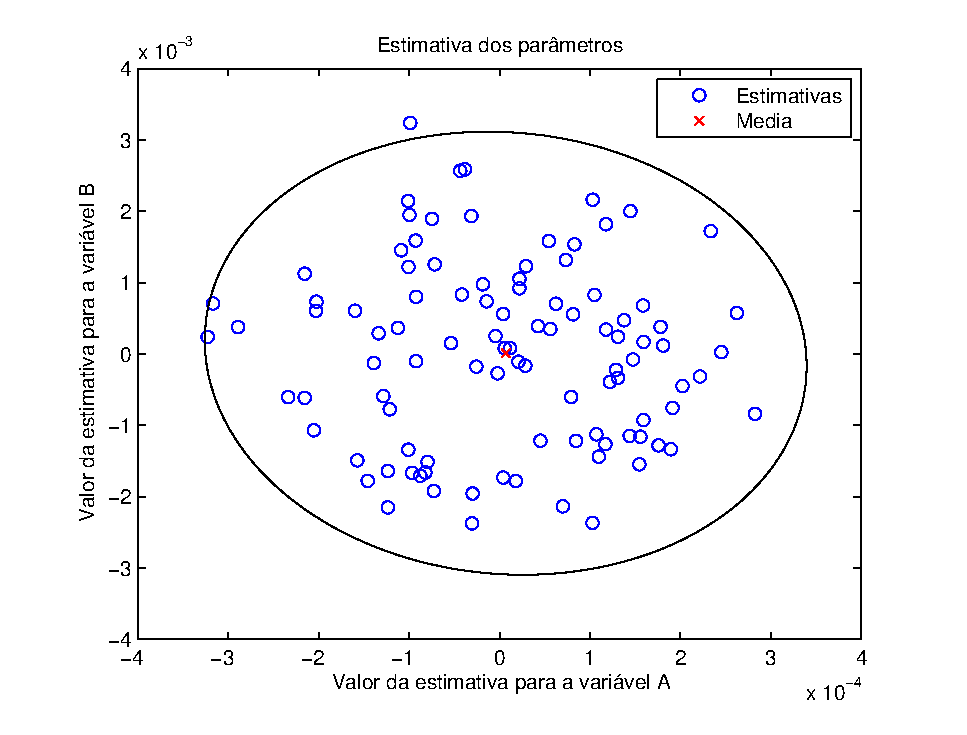
\includegraphics[width=0.8\columnwidth]{figures/si_covar_elipse.eps}
	\caption{Estimativas de um sistema e a regi�o de confian�a para $\chi$ de 95\%}
	\label{fig:si_covar_elipse}
\end{figure}


%===============================================================================
\section{Projeto de Experimento}
\label{sec:si_project_experiments}
%===============================================================================

Projeto de experimentos pode ser entendido como o procedimento para que se escolha o melhor 
sinal de entrada para a identifica��o dos par�metros desejados para o experimento. 
Desta forma muitas vari�veis podem ser levadas em considera��o, refletindo em propriedades que
podem ou n�o ser o foco do projeto de experimentos.

Uma forma de organizar o projeto de experimento � desenvolve-lo como um problema de otimiza��o 
convexa, onde entre muitas vantagens est� o fato de que � poss�vel a utiliza��o de m�todos matem�ticos
para o seu c�lculo e sua formula��o pode ser feita por LMI ({\it{Linear Matrix Inequality}}. Em \cite{jasson}
este t�pico � explorado em mais profundidade, sendo aqui apenas apresentado a sua ideia b�sica.

%===============================================================================
\subsection{Modelagem como um problema de otimiza��o}
\label{sec:si_project_optimization}
%===============================================================================

O problema de projeto de experimento pode ser considerado como uma forma geral apresentada em \eqref{eq:si_project_optimization}

\begin{equation}
\begin{matrix}
\underset{\Phi_{\chi_0}}{\text{minimize}} &  & \text{Objetivo}\\ 
\text{Sujeito a:} &  & \text{Requisitos de qualidade}\\ 
 &  & \text{Requisitos de sinais}
\end{matrix}
\label{eq:si_project_optimization}
\end{equation}

De forma geral os requisitos de qualidades s�o fun��es da covari�ncia de $P$. Por esta raz�o � natural usar
o espectro da entrada $\Phi_u$ e eventualmente o espectro cruzado $\Phi_{ue}$ como vari�veis do projeto.
A inclus�o de limita��es nos sinais e sua inclus�o como vari�veis de projeto s�o �teis para evitar que se chegue
em resultados onde a energia de entrada precise ser infinita para se obter os crit�rios desejados, ou largura
de banda que n�o s�o facilmente ating�veis em projetos reais. \cite{jasson}



%===============================================================================
\section{Considera��es Finais}
\label{sec:si_conclusions}
%===============================================================================

%===============================================================================


